\documentclass[a4paper,12pt]{article}
\usepackage{blindtext}
\usepackage[utf8]{inputenc}
\usepackage{graphicx}
\usepackage{array}
\newcolumntype{L}{>{\raggedright\arraybackslash}m{8cm}}

\begin{document}
\begin{titlepage}
\center

\textsc{\LARGE Software Requirements Specification}\\[1.5cm]
\textsc{\Large Project: NavUP}\\[0.5cm]
\textsc{\large Team: Wheat}\\[0.5cm]

\begin{minipage}{0.4\textwidth}
\begin{flushleft} \large
\emph{Author(s):}\\
Xolo \textsc{Dandashe}\\
Mia \textsc{Gerber}\\
Hlengekile \textsc{Jita}\\
Brian \textsc{Ndung'u}\\
Nathan \textsc{Ngobale}\\
Takalani \textsc{Sigama}\\
\end{flushleft}
\end{minipage}
~
\begin{minipage}{0.4\textwidth}
\begin{flushright} \large
\emph{Student number(s):} \\
14245681\\ % Student number
15016502\\
14077893\\
15322913\\
15110045\\
14166365\\
\end{flushright}
\end{minipage}\\


\includegraphics[width=\textwidth]{images/up_logo.jpg}

{\large University of Pretoria, Department of Computer Science}\\[0.5cm]
{\large 24 February 2017}\\[3cm]

\vfil
\end{titlepage}

\newpage
\tableofcontents
\newpage

\section{Introduction}
\subsection{Purpose}
The purpose of this Software Requirements Specification(SRS) document is to provide a high level specification of the NavUP system. This document will fully describe the NavUP systems behaviour by detailing its functional and non-functional requirements. The intended audience of the document is all parties that will be involved in the project from the planning to the testing phase, this includes, designers, developers, users and more.
\subsection{Scope}
The system to be developed is called \textit{\textbf{NavUP}}. NavUP is a Navigation system for the University of Pretoria. Hence the name NavUP, Navigation UP. \\

NavUP will help numerous people who partake in activities on campus. This includes students, lecturers, workers and guests on campus. The system will not only help them maneuver around campus but also get them better acquainted with numerous aspects of the UP campus. The main task of NavUP will be providing a navigation system for the UP campus. This includes identifying locations, identifying points of interest and places where activities are taking place and providing directions to those places. This can be classes, events that take place on campus, and transportation routes such as the UP buses drop off and pick up locations, restaurants and shops on campus.

In addition the system should also be able to determine optimal routes for users to take based on their preferences as well as by avoiding pedestrian traffic, which is a common occurrence on campus. To further enhance the experience of users of the system, additional features, such as including the users campus timetable and providing directions to locations at scheduled times and counting their number of steps per day and comparing it to other users, will be included. 

The system will interface with other systems in order to achieve its purpose. These systems are namely the WiFi system currently available at UP and device GPS systems.

\subsection{Overview}
The rest of the SRS document is organized as follows, firstly we provide an overall description which is an overview of the NavUP system. This describes the NavUP product as a whole and gives a brief description of its various interfaces and requirements, its functions, the users of the system as well as constraints and assumptions that will affect the system. Secondly we describe the software requirements of the system. This includes both the functional and non-functional requirements.

\section{Overall Description}
\subsection{Product Perspective}
\subsubsection{System Interfaces}
The NavUP will have the following system interfaces as shown in the following figure\\
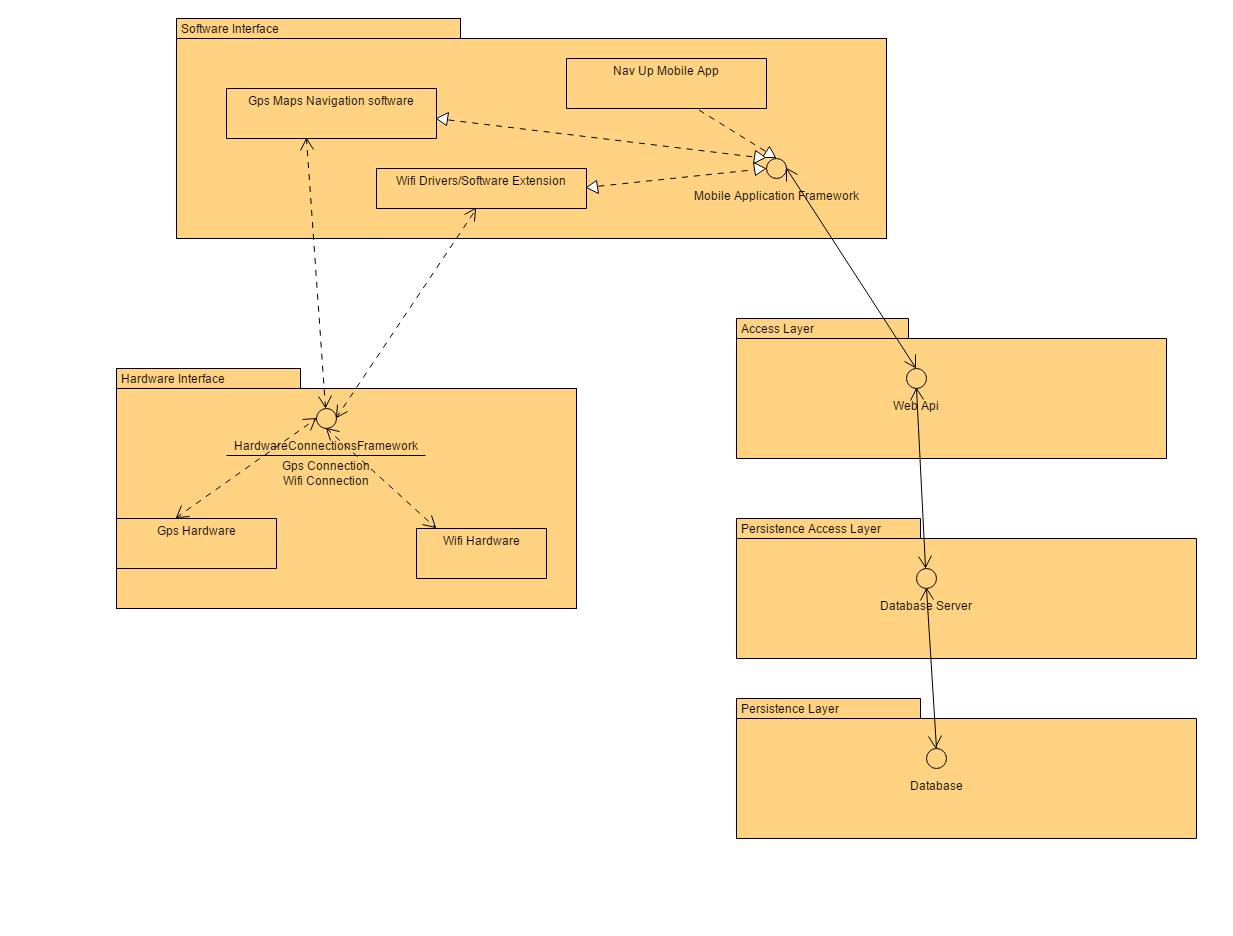
\includegraphics[width=\textwidth]{images/system_interface.png}
\textbf {Client Interface}\\
Users of the system will use a mobile application which requires a mobile device. This hardware device will either be a smart phone or a tablet and will need to have GPS and WiFi capabilities. On this device we will run an application which is our software interface which will either be the Web, Android or iOS application. These applications will access the GPS software and WiFi of the phones and interact with the server where most functionality will take place before the results are pushed back to the user.\\
\textbf{Web Server}\\
The Web Server will handle the back-end operations of the system. This will include the business processes and the CRUD database operations necessary to provide the users with the functionality. The Web Server will also be responsible for triangulating WiFi signals to pinpoint locations and any other  back-end operations \\
\textbf{Database}\\
The database will be responsible for storing all necessary persistent information. This will include but is not limited to location data, WiFi router data and user data.
\subsubsection{User Interfaces}
For this application, mobile devices like smart phones and tablets will be used. This will serve as the interface between the user and the system. Mobile applications, Android and iOS, and a Web Application will be designed for these devices, these applications will provide the users with a Graphical User Interface(GUI). A variety of screens will be shown to the user in order to provide them with information and allow them to interact with the NavUP system. These screens will be designed to give them the best user experience possible. Following, we give mock-ups of the user interface and describe some of the interactions the user should be able to make with the system. 

The user will be able to set their starting position either by setting it themselves or by use of the system's ability to determine their current position. This is demonstrated in the mock-up shown in fig. 1, the user can use this interface to set a destination and also use their previously set or visited destinations. \\
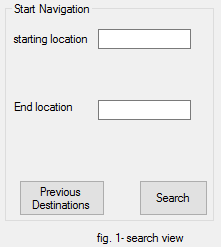
\includegraphics[scale=1]{images/user_one.PNG}\\
Once the user is ready to search they are transferred to the screen displayed by the mock-up in fig. 2 where they can choose their desired route. Options are given to the user to select which route they prefer. They will also be given an option to get an optimal route that will  take into consideration user preferences and get the user to their destination the quickest and shortest way possible with the least traffic. Once the route is selected the user can choose to begin the navigation.\\
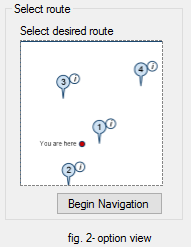
\includegraphics[scale=1]{images/user_two.PNG}\\
A visual representation of the location of the user is given while they are en-route to their destination as show in the mock-up in fig. 3. Push notifications are sent to the user to let them know which direction should take. Total steps, distance and time taken to reach their destinations is tracked. These statistics are used to give the user goals to achieve. This is shown in the mock-up in fig. 4. A timetable integration feature will also be included which will give the user directions to classes at appropriate times, as shown in the mock-up in fig. 5. \\
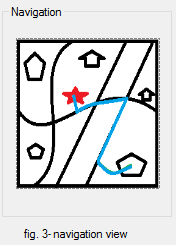
\includegraphics[scale=1]{images/user_three.PNG}
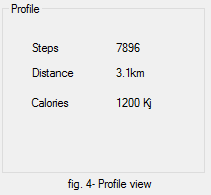
\includegraphics[scale=1]{images/user_four.PNG}
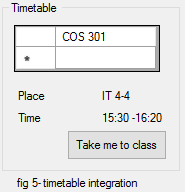
\includegraphics[scale=1]{images/user_five.PNG}\\
\subsubsection{Hardware Interfaces}
The minimum hardware device required mainly is a mobile device either a cellphone or a tablet, that has WiFi, GPS and Internet connectivity capabilities. The system will be run using iOS and Android applications on the mobile devices. For best results with Apple devices they should be running iOS 8 or newer. For best results with other smart phones, they should be running Android version 5.0 or newer. 
\subsubsection{Software Interfaces}
The NavUP application communicates with the connected WiFi router in order to get geographical information about where the user is located and then visually represents it on the user's device. Once the current location is found, the application waits for the user to input a target destination then starts to calculate routes. 

During calculation all possible routes are determined by discerning pathways, checking most traveled route and checking pedestrian traffic. The user is then given the option to select the route they want to take, once the route is selected then navigation begins. Directions are given to the user as they are en-route and their walking statistics are recorded for their profile. The diagram below shows this interaction between the user and the application. Hence the software interfaces of the system will need to be able to provide the user with the above described functionality.\\
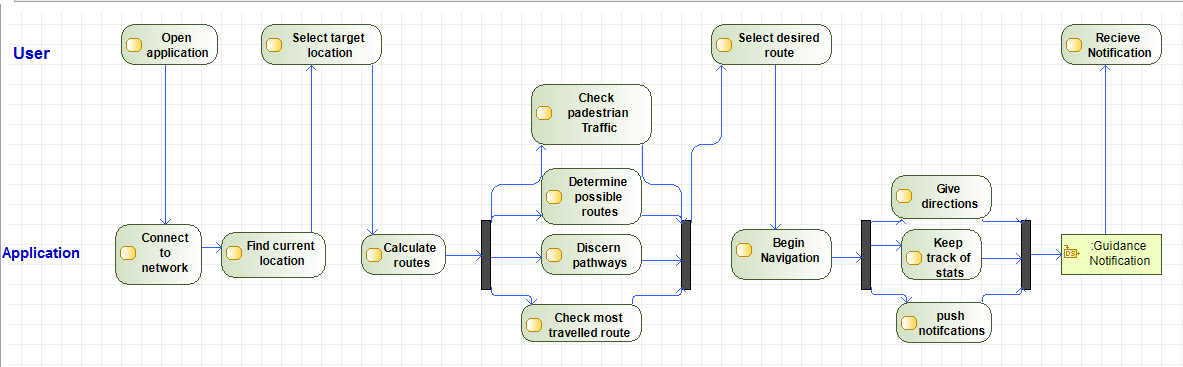
\includegraphics[width=\textwidth]{images/software_interface.png}\\
\subsubsection{Communications Interfaces}
%Future work
\subsubsection{Memory}
%Future work
\subsubsection{Operations}
%Future work
\subsubsection{Site Adaption Requirements}
%Future work
\newpage
\subsection{Product Functions}

\begin{table}[!htbp]
\centering
\footnotesize
\label{tab:table 2.2}
\bgroup
\def\arraystretch{1.3}
\begin{tabular}{|L|L|}
\hline
FUNCTION & DESCRIPTION 
\\
\hline
Corrects/recalculates the path if the user is not following the route correctly. & If the user takes a wrong turn, the application will send a push notification to the user’s device, telling them that they are no longer on the correct route. The user can then either choose to recalculate the route and follow the new path or they can ask to be directed back to the original path. 
\\
\hline
Users can search for a building/location and the system will find it. & The name that the user requested can be mapped to a physical location on the UP campus. (The coordinates of specific buildings are associated with the name of the building)
\\
\hline
The user can specify a current location and destination using the search facility. & The current location and destination are saved so that it can be used to determine the route later on. 
\\
\hline
The user can use parameters so that the application can choose the optimal route for their purposes. & The application will provide several routes that the user can take to arrive at their destination, then choose from the routes generated the path that matches the criteria given by the user e.g. “shortest route” or “route that has a bathroom along the way”
\\
\hline
The application gives step by step directions on how to reach your destination & The application in real time tracks where the user is currently walking and then gives them instructions either as push notifications or audio when it is needed so the user stays on the plotted route, for example "turn left" or "take the stairs to the fourth floor". 
\\
\hline
The user can put their schedule into the application and it will generate a route for the whole day & The application will use your personalized timetable to determine a path that has every class you are going to that day along the route so that you don’t have to continually generate routes.
\\
\hline
The application tracks distance walked & You will get daily/weekly/monthly push notifications informing you of how far you have walked since a certain point in time (you can specify when the app should start calculating distance.)
\\
\hline
The application tracks which users have walked the furthest in a specific day/week/month. & The distance data from all users will be consolidated and a leader board will be created showing the top 5 students.
\\
\hline	
\end{tabular}
\egroup	
\end{table}

\subsection{User Characteristics}
\begin{itemize}
\small
\item Users will be both male and female
\item Users are university students ranging in age from 18 to 25
\item Users come from a vast array of different cultural and economic backgrounds
\item Users have graduated high school and have a median level of literacy
\item Users communicate in English using UK grammar and spelling conventions.
\item Users have used mobile devices before and are familiar with touchscreen interfaces
\item Users understand the basic concept of a wireless network and how to connect to it using a mobile device
\item Users will be both new students (no prior knowledge of the campus) and existing students (possess existing knowledge of campus)
\item Users might have disabilities, developers need to be conscious of this when designing the application. 
\end{itemize}
\subsection{Constraints}
\paragraph*{What restrictions will affect development?} 
The project requires that the application be implemented using the WiFi network on campus to determine the location of users, but because the signal strength and coverage of the network is not uniform across campus, this can severely impact the accuracy of the application and how useful it will end up being.
\\
Continuing on from the previous constraint, we can assume that because there is not WiFi available in every single part of campus, sometimes the application will have to revert to using mobile data. Students will be using the application which means our application needs to use minimal mobile data. Designing data transfer that does not use a lot of mobile data is difficult and will require us to restrict the amount of real-time data transfer that is done by the application or to implement it in a way that means they are able to use the application offline for short periods of time.  
\\
The experience of the development team may also end up becoming a constraint, the amount of features and functionality we are able to deliver on will depend largely on our technical skill level and whether we are able to come up with elegantly simple solutions.
\\
We need to ensure that this application is deployed on all mobile platforms for all mobile devices (phones, tablets, laptops etc) this means we are unable to use platform specific technologies which limits the amount of solutions we will be able to produce. 
\\
User privacy needs to be taken into account as a constraint on development. Some historical data about the user will need to be stored, but the type of data we are allowed to store will dictate which functionality we are able to bring about in the application. For example, instead of showing you your 5 most visited places, the application will only tell you how many steps you've taken in a day. 
\\
\subsection{Assumptions and Dependencies}
\begin{enumerate}
\item We are assuming that users will have the WiFi setting on their phones enabled at all times, our entire navigation system depends on this assumption because checking how the user's device connects to different routers as they move through campus is critical to determining their current location. 
\item We are assuming that the location of every WiFi router in the network is known and has been mapped onto a schematic of the Hatfield campus. We need to be able to locate the router that a user is connected to.
\item To generate a heat map of the traffic conditions on campus (where the highest concentration of people currently are) we will need to assume that all students on campus both have the application downloaded and running while they are moving around on campus.
\item All possible solutions outlined in this document will work on the assumption that we have not been given any limit on the size of our database or the capacities of the server that will be used.
\end{enumerate}

\section{Specific Requirements}
\subsection{External Interface Requirements}
%Future work
\subsection{Functional Requirements}
\subsubsection{System Modules}
\textbf{1. Locations}\\
This module will be responsible for everything location related. It will store data about locations such as GPS coordinates, it's name, whether its a point of interest or not. This module will also be responsible for storing user specified locations and provide services such as determining their current location and finding locations. This module will also store the UP calendar and allow the updating of event and activity locations. Some of the functionality provided by this is as follows:
\begin{itemize}
\item \textbf{GetLocation -} This function retrieves the GPS coordinates of a certain location. This is a critical function.
\item \textbf{SearchLocation -} This function searches for a location and if found returns its GPS coordinates. This function is critical
\item \textbf{SaveLocation -} This function saves a location. This function is important.
\item \textbf{GetActivity -} This function gets an activity available on campus and provides the user with its time and location. This function is nice-to-have.
\end{itemize}

\textbf{2. Routes}\\
This module will be responsible for determining routes and providing navigation between locations. The module will determine all routes from locations as well as determine the optimal route. This module will also display the user with a map as they navigate their way around campus. The module will also store most requested routes and the routes between frequently visited locations. Routes will be identified using their starting and end locations. Some of the functionality provided by this module will be:
\begin{itemize}
\item \textbf{GetDirections -} This function determines the routes from one place to another. This function is critical.
\item \textbf{StoreRoute - } This function will store a route when it is frequented often. This function is important.
\item \textbf{GetStoredRoute - } This function will fetch a stored route. This function is important.
\end{itemize}

\textbf{3. Traffic}\\
This module will be responsible for traffic. This is the surveillance and determination of traffic conditions whether by using cameras or crowd-sourcing. This module will also store which locations are usually heavily populated and at what times. This module will also push traffic notifications to users who request it. In addition to that, users currently using the map to navigate will also be provided with a heat map that displays traffic conditions to them. Some of the functionality provided by this module is described:
\begin{itemize}
\item \textbf{DetermineTraffic -} This function determines the traffic on a specified route. This function is important.
\item \textbf{ShowTraffic -} This function displays the traffic conditions to the user. This function is nice-to-have.
\end{itemize}

\textbf{4. Users}\\
This module will be responsible for user information. This will store user information such as log in credentials, if they participate in activities, user schedules, user preferences and other information. This module will be responsible for providing the users preferences while using the application to get routes and navigation. This module will also be used by activities to update user information and enable interaction among other users. Some of the functionality provided by the module are: 
\begin{itemize}
\item \textbf{CheckUserCredentials -} This function checks inputted user credentials against stored credentials to authenticate users. This function is important.
\item \textbf{GetUserLocation -} This function gives the users current location in GPS coordinates. This function is critical.
\item \textbf{GetPreferences -} This function gets the users preferences. This function is important.
\item \textbf{SetPreferences -} This function sets and stores the users preferences. This function is important.
\end{itemize}

\textbf{5. Activities}\\
This module will be centered around extra features of the application not centered around navigation. This will include activities such as steps taken, calories burnt, distance covered and the like. This module could also include a explore campus function which takes the user around campus to discover new things by selecting random locations. This module will allow interaction between users.
 
\textbf{6. Notifications}\\
This module will be responsible for notifying users. This module will require scheduling functionality in order to push notifications at appropriate times. Notifications will be requested by other modules and will set up the information required for the notification. Some of the functionality to be provided by this module is:
\begin{itemize}
\item \textbf{NotifyUser -} This function sends push notifications to the user. This function is nice-to-have.
\end{itemize}

\subsubsection{Use Cases}
In this section, we describe each key feature that the system shall provide and the functional requirements for that feature. The functional requirements are the functions, inputs and outputs required for a feature or use case to be achieved. \\

\textbf{\large FindVenue Use Case}\\
\textbf{Description: } This use case helps the user to find a venue on campus\\
\textbf{Priority Level: } Critical\\
\textbf{Inputs:} Name of venue\\
\textbf{Outputs:} Location of inputted venue\\
\textbf{Use case diagram: }\\
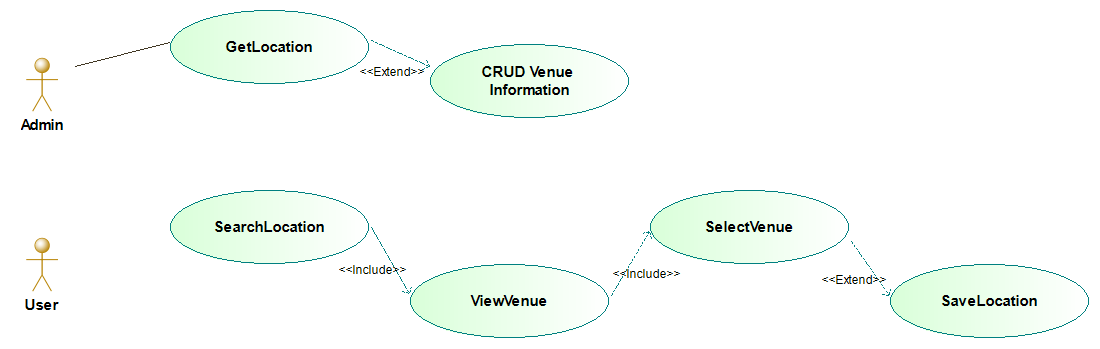
\includegraphics[width=\textwidth]{images/find_venue.png}


\textbf{\large FindService Use Case}\\
\textbf{Description: } This use case helps the user to find a service that is available on campus\\
\textbf{Priority Level:} Important\\
\textbf{Inputs:} A service\\
\textbf{Outputs:} Location of inputted service\\
\textbf{Use case diagram: }\\
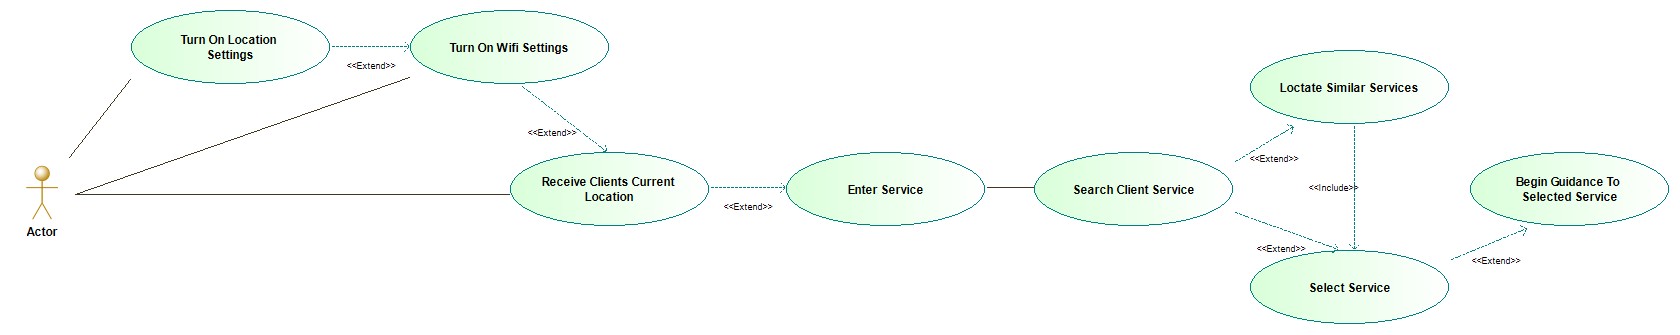
\includegraphics[scale=1, width=\textwidth, height=5cm]{images/find_service.png}

\textbf{\large ProvideRoute Use Case}\\
\textbf{Description: } This use case provides a route from a location on campus (which could be the user's current location or specified) to another location on campus (which could be specified or returned by FindVenue or FindService).\\
\textbf{Priority Level: } Critical\\
\textbf{Inputs:} From Where and To Where\\
\textbf{Outputs:} Route from a place to another place\\
\textbf{Use case diagram: }\\
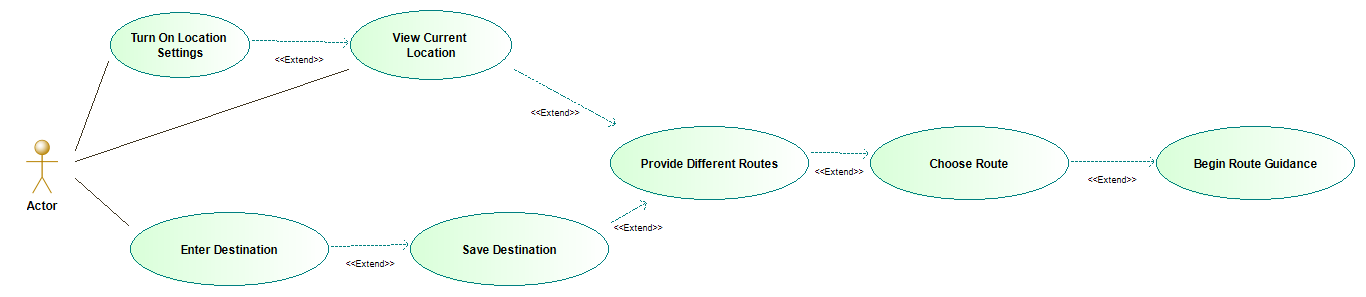
\includegraphics[width=\textwidth]{images/provide_route.png}

\textbf{\large ProvideOptimalRoute Use Case}\\
\textbf{Description: } This use case provides the best route from a location on campus to another location on campus. "Best" route being determined by user specified factors such as if traffic should be avoided or if the student center should be passed on the way\\
\textbf{Priority Level: } Important\\
\textbf{Inputs:} From Where, To Where and User Preferences\\
\textbf{Outputs:} Optimal route from a place to another place\\
\textbf{Use case diagram: }\\
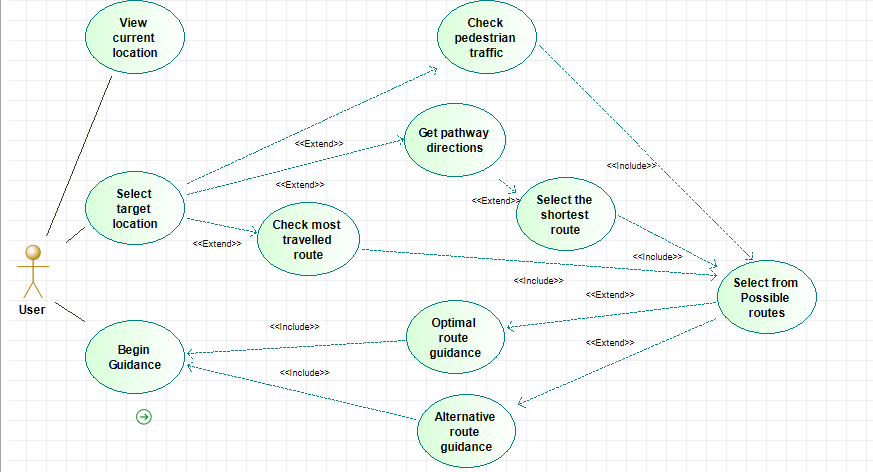
\includegraphics[width=\textwidth]{images/op_route.png}

\newpage
\subsubsection{Actor-System Interaction}
\begin{table}[!htbp]
\footnotesize
\label{tab:table 3.2.3}
\bgroup
\def\arraystretch{1.3}
\begin{tabular}{|L|L|}
\hline
\textbf{\textit{ACTOR - USER}} & \textbf{\textit{SYSTEM - UP NAV}}
\\
\hline
\textbf{1.} User opens application \linebreak \linebreak
\textbf{Precondition:} User does not know how to get somewhere. & \textbf{2.} Application opens on mobile device and lists all options for navigation. \linebreak \linebreak
\textbf{Precondition:} No user input has been given so a default screen is displayed.
\\
\hline
\textbf{3.} User successfully identifies the navigation option from start menu \linebreak \linebreak
& \textbf{4.} System prompts user for destination to navigate to. \linebreak \linebreak
\textbf{Postcondition:} After determining the user's location it can start searching for possible path for the destination.
\\
\hline
\textbf{5.} User adds a criteria (e.g. avoid traffic) to refine the route \linebreak \linebreak
\textbf{Postcondition:} Adding extra information results in a better path.
& \textbf{6.} System chooses a single route and prepares step-by-step instructions to deliver to the user telling them how to arrive at their destination. \linebreak \linebreak 
\textbf{Postcondition:} The GUI will display the route to the user and real-time navigation will begin as the user starts following the given directions.
\\
\hline
\textbf{7.} User follows push notifications and prompts along the chosen route \linebreak
& \textbf{8.} System tracks the user's movement, checking whether their movements correspond to the path given. \linebreak
\\
\hline
\textbf{9.} User strays from given route \linebreak \linebreak
\textbf{Postcondition:} User is no longer following the route and might not arrive at destination.
& \textbf{10.} Constantly tracking the user as he/she moves the application can see that the user is no longer on route and will prompt the user to go back onto the original path or suggest alternatives to follow. \linebreak \linebreak
\\
\hline
\textbf{11.} User gets back onto the right route and arrives at destination \linebreak \linebreak
\textbf{Precondition:} The user was following the wrong path \linebreak 
\textbf{Postcondition:} The user now follows the path that will lead to their destination.
& \textbf{12.} System alerts user that they have arrived at their destination through some visual feedback and exits the navigational mode. \linebreak
\\
\hline	
\end{tabular}
\egroup	
\end{table}

\subsubsection{Traceability Matrix}
The traceability matrix visually depicts the functional requirements and their priority in relation to the use cases and their priority. \\
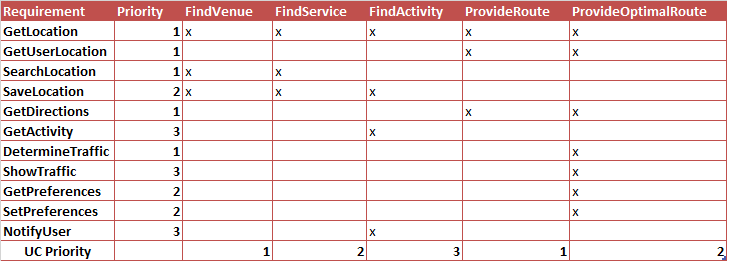
\includegraphics[width=\textwidth]{images/trmatrix.png}

\subsection{Performance Requirements}
\begin{itemize}
\small
\item The system should provide the relevant location searched for by the user within a short amount of time.
\item The system should provide the accurate location of the user inside or outside of a building using WiFi connectivity.
\item The system should be able to provide the most effective or quickest route from the users location to their specified destination.
\item The system should be resource friendly and not significantly impact the battery life of the device it is on.
\item The system should be able to be paused and continued.
\item The system should also be able to accommodate the student population and guests so that the number of users using the system will not hinder the performance of the application.
\end{itemize}
\subsection{Design Constraints}
\begin{itemize}
\small
\item Limited WiFi hotspots will affect the accuracy of determining the users location.
\item Different WiFi standards on devices would affect the accuracy of triangulating a users location.
\item The dependence on the WiFi hotspots means that if it were to experience some form of failure the system will as a result also fail.
\item Different device displays could affect the way in which the navigation system will be displayed on different devices.
\item The size of the system on memory should be taken into consideration to allow for as many devices as possible, therefore it has to be resource friendly.
\end{itemize}
\subsection{Software System Attributes}
\begin{itemize}
\small
\item The reliability of the system will be dependent on the accuracy of determining the users location and destination and providing accurate and effective routes.
\item The security of the system would be the safety protocols to prevent any misuse of users private information which in this case would be their location. These safety protocols include forms of encryption in the database and access control for administrative purposes.
\item The availability of the system is another crucial attribute which determines the quality of the system. The system should be readily available at any time to assist the user with navigation. 
\item The interoperability of the system should allow for the communication amongst multiple devices made by different manufacturers in order to effectively use that information for crowd sourcing purposes and in order to identify congested areas.
\end{itemize}
\subsection{Other Requirements}
\begin{itemize}
\small
\item The system should also gamify the experience to make it more interactive and enjoyable in order to promotes its usage.
\item The system should be able to apply some form of machine learning to provide relevant information to the user in relation to possible events or interests that the user could possibly be interested in.
\end{itemize}
\section{Appendix}
\subsection{Glossary of terms}
%Explanations of terms
%Definitions, Acronyms, Abbreviations
\subsection{References}
%Software Engineering textbook, more if any
\section{Index}

\end{document}